\chapter{Geometry}
    \section{Simple Geometry}
    This section will have alot of functions used in geometry problems. They are related to points, lines, circles and polygons.
    \subsection{Points and Lines}
    This is the base of all codes in geometry. u can change the type from ldb to ll and also change the EPS. The rest is pretty much fixed.
    \lstinputlisting{./solutions/Geometry/base.cpp}
    \subsection{Circles}
    This section will have alot of algorithms related to circles and their description
    A circle will have the following format:
    \begin{lstlisting}
    typedef pair<pt, T> circle;
    \end{lstlisting}
    
    
    To see if a point is in/on/out a circle we can do:
    \begin{lstlisting}
// -1 if inside, 0 if in border, 1 if outside
int in(const circle& x, const pt& y) { 
    return sgn(abs(y-x.ft)-x.sd); 
 }
    \end{lstlisting}
    Arc length of two points:

    \begin{center}
    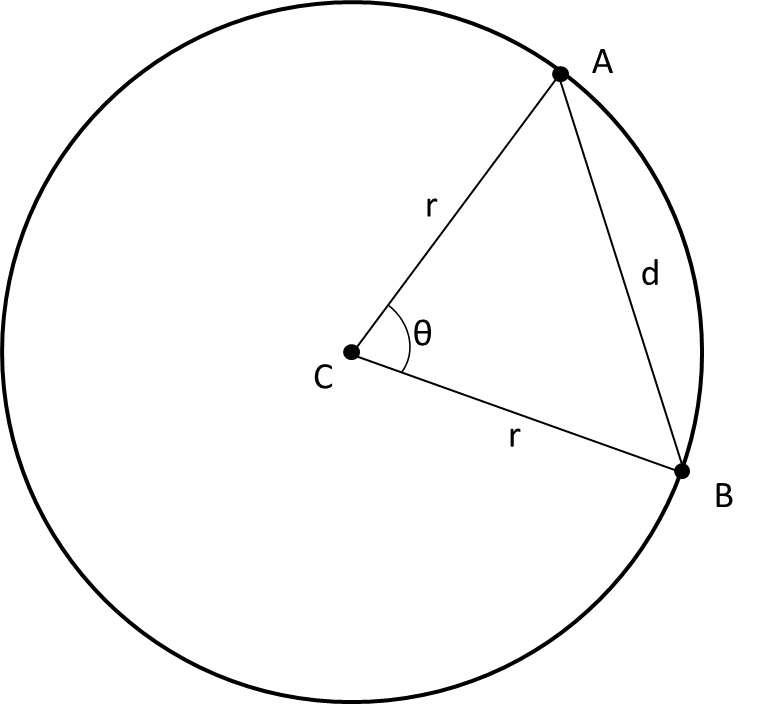
\includegraphics[scale = 0.5]{imgs/arclength.png}
    \end{center}
    
    \begin{lstlisting}
T arcLength(const circle& x, pt a, pt b) {
    // precondition: a and b on x
    pt d = (a-x.ft)/(b-x.ft); return x.sd*acos(d.ft); 
}
    \end{lstlisting}
    
    Intersections related to circles:
    \begin{lstlisting}
vpt isect(const circle& x, const circle& y) { // precondition: x!=y
    T d = abs(x.ft-y.ft), a = x.sd, b = y.sd; 
    if (sgn(d) == 0) { assert(a != b); return {}; }
    T C = (a*a+d*d-b*b)/(2*a*d); 
    if (abs(C) > 1+EPS) return {};
    T S = sqrt(max(1-C*C,(T)0)); 
    pt tmp = (y.ft-x.ft)/d*x.sd;
    return {x.ft+tmp*pt(C,S),x.ft+tmp*pt(C,-S)};
}

vpt isect(const circle& x, const line& y) {
    pt c = foot(x.ft,y); 
    T sq_dist = sq(x.sd)-abs2(x.ft-c);
    if (sgn(sq_dist) < 0) return {};
    pt offset = unit(y.sd-y.ft)*sqrt(max(sq_dist,T(0)));
    return {c+offset,c-offset};
}

T isect_area(circle x, circle y) { // not thoroughly tested
    T d = abs(x.ft-y.ft), a = x.sd, b = y.sd; 
    if (a < b) swap(a,b);
    if (d >= a+b) return 0;
    if (d <= a-b) return PI*b*b;
    T ca = (a*a+d*d-b*b)/(2*a*d), cb = (b*b+d*d-a*a)/(2*b*d);
    T s = (a+b+d)/2, h = 2*sqrt(s*(s-a)*(s-b)*(s-d))/d;
    return a*a*acos(ca)+b*b*acos(cb)-d*h;
}
    \end{lstlisting}

    A tangent to a circle is a line in the plane of a circle which intersects the circle in exactly one point. This point is called the point of tangency.

    A tangent of two circles is a common internal tangent if the intersection of the tangent and the line segment joining the centers is not empty.

    \begin{center}
    \begin{minipage}{.5\textwidth}
    \centering
    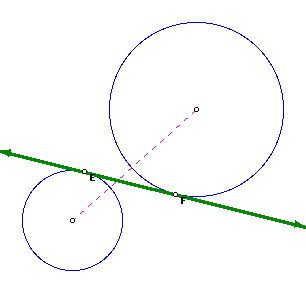
\includegraphics[scale = 0.5]{imgs/internal1.png}
    \end{minipage}%
    \begin{minipage}{0.5\textwidth}
    \centering
    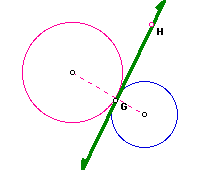
\includegraphics[scale = 0.5]{imgs/internal2.png}
    \end{minipage}
    \end{center}
    
    
    A tangent of two circles is a common external tangent if the intersection of the tangent and the line segment joining the centers is empty.

    
    \begin{center}
    \begin{minipage}{.5\textwidth}
    \centering
    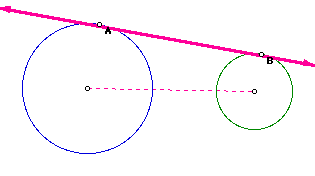
\includegraphics[scale = 0.5]{imgs/external1.png}
    \end{minipage}%
    \begin{minipage}{0.5\textwidth}
    \centering
    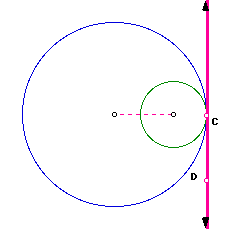
\includegraphics[scale = 0.5]{imgs/external2.png}
    \end{minipage}
    \end{center}
    
    \begin{lstlisting}
pt tangent(pt x, circle y, int t = 0) {
	y.sd = abs(y.sd); // abs needed because internal calls y.s < 0
	if (y.sd == 0) return y.ft;
	T d = abs(x-y.ft);
	pt a = pow(y.sd/d,2)*(x-y.ft)+y.ft;
	pt b = sqrt(d*d-y.sd*y.sd)/d*y.sd*unit(x-y.ft)*dir(PI/2); 
	return t == 0 ? a+b : a-b;
}
vector<pair<pt,pt>> external(circle x, circle y) { 
	vector<pair<pt,pt>> v; 
	if (x.sd == y.sd) {
		pt tmp = unit(x.ft-y.ft)*x.sd*dir(PI/2);
		v.eb(x.ft+tmp,y.ft+tmp);
		v.eb(x.ft-tmp,y.ft-tmp);
	} else {
		pt p = (y.sd*x.ft-x.sd*y.ft)/(y.sd-x.sd);
		rep(i, 0, 2) v.eb(tangent(p,x,i),tangent(p,y,i));
	}
	return v;
}
vector<pair<pt,pt>> internal(circle x, circle y) { 
	return external({x.ft,-x.sd},y); }
    \end{lstlisting}

    The CircumCenter of a triangle is the minimum enclosing circle of a triangle.
    We can also calculated the minimum enclosing circle of a polygon.

    \begin{center}
    \begin{minipage}{.3\textwidth}
    \centering
    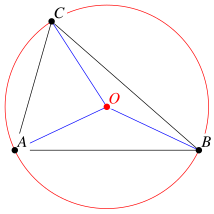
\includegraphics{imgs/circumcenter.png}
    \end{minipage}%
    \begin{minipage}{0.7\textwidth}
    \centering
    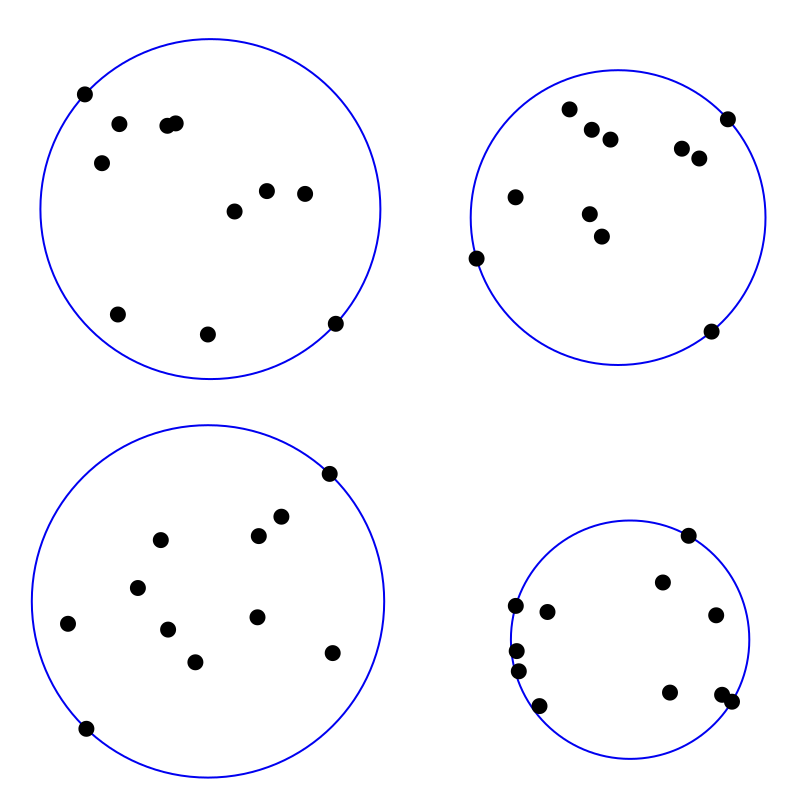
\includegraphics[scale = 0.5]{imgs/mec.png}
    \end{minipage}
    \end{center}
    

    
    \begin{lstlisting}
// return the minimum enclosing circle of a triangle
circle ccCenter(pt a, pt b, pt c) { 
	b -= a; c -= a;
	pt res = b*c*(conj(c)-conj(b))/(b*conj(c)-conj(b)*c);
	return {a+res,abs(res)};
}

// return the minimum enclosing circle of a set of points O(N)
circle mec(vpt ps) {
	shuffle(all(ps), rng);
	pt o = ps[0]; 
    T r = 0, EPS = 1+1e-8;
	rep(i, 0, (int)ps.size()) 
        if (abs(o-ps[i]) > r*EPS) {
            o = ps[i], r = 0; // point is on MEC
            rep(j, 0, i) 
                if (abs(o-ps[j]) > r*EPS) {
                    o = (ps[i]+ps[j])/2, r = abs(o-ps[i]);
                    rep(k, 0, j) if (abs(o-ps[k]) > r*EPS) 
                        tie(o,r) = ccCenter(ps[i],ps[j],ps[k]);
                }
        }
	return {o,r};
}
    \end{lstlisting}
    \section{Convex Hull}
        \subsection{Rotation Calipers}
        Diameter from a convex Polygon.
        
        Solution $O(n)$. Original Problem (NCPC 2013 - D).
        
        \ \\
        
        \begin{tabular}{|p{31cm}|}
          \begin{verbatim}
            Implementacao do Convex Hull do CP-ALGORITHMS
            Para usar crie um vetor com os pontos,
            		vector<pt> pts;
            e execute
            		convex_hull(|pts|);
            Apos isso, o vector pts sera alterado e ele so tera os pontos do Convex Hull 
            na ordem horaria, comecando do elemento de menor x, como segunda condicao menor y.
            
            Como funciona o algoritmo
            - Acha os dois extremos de x.
            - Monta dois subgrupos, os "up" e os "down", em relacao
            Convex Hull na parte superior e inferior.
            - Itera pelos pontos e usa o produto vetorial para ver se
            ele forma um sentido horario, se formar adiciona.
            - Remove todos os anteriores ao ultimo ponto adicionado que agora, com o ponto
            atual, formando um sentido anti-horario
            \end{verbatim}
        \end{tabular}
        \\
        
        \lstinputlisting{./solutions/Geometry/MaxDistanceBetweenPoints.cpp}
        
    \section{Line Sweep}
        \subsection{Points Inside Triangles}
        Given $n$ triangles with vertices {($x_i$, $y_i$), ($x_i + d$, $y_i$), ($x_i$, $y_i + d$)}, and $q$ points, compute for each triangle, the number of points that lie inside or in boundary of him. $O(nlogn)$. (Original Problem: CODECHEF - TRIANGULAR QUERIES)
        \lstinputlisting{./solutions/Geometry/PointsInsideTriangles.cpp}
        \newpage
        \subsection{Ranking Problem}
        Given $n$ students that attended to $3$ contests, and all of them have different ranks, between $1$ and $n$ inclusive, for each contest. We say that one student $a$ is better that student $b$, if all ranks of student $a$ in each contest is lesser that student $b$. A student is said to be excellent if no other student is better than him. How many excelent students there exists ?
        
        This solutions runs in $O(nlogn)$. (Original Problem: SPOJ: NICEDAY)
        
        \lstinputlisting{./solutions/Geometry/RankingProblem.cpp}
        \newpage
        \subsection{Balls Falls and Segments}
        Given $n$ segments (non horizontal and with no common points), and $m$ balls in a 2D plane, say for each ball the x point which he falls. (This solution was upload, the source code is just for only one ball, but the overall complexity is still $O(nlogn)$ if the number of balls is $O(n)$).
        
        This solutions runs in $O(nlogn)$. Original Problem (NCPC 2013 - H).
        
        \lstinputlisting{./solutions/Geometry/WaterFalls.cpp}
        \newpage
        \subsection{Checking Points Inside Convex Polygon}
            % \subsubsection{Offline}
            % Given $n$ points in 2D plane, and a Convex Polygon, check for each of these $n$ points, if them are strict inside or not of polygon.
            
            % This solutions runs in $O(nlogn)$ but i used Fracion Class to Take Care with double error precisions, so the overall solution in this case is $O(nlogn^2)$.
            
            % \lstinputlisting{./solutions/Geometry/PointsInsideConvexPolygon.cpp}
            % \newpage
            \subsubsection{Online}
            Given one point and a Convex Polygon, with vertices in counter clockwise order, check if this point is inside or in boundary of him.
            
            This solutions runs in $O(logn)$.
            
            \lstinputlisting{./solutions/Geometry/PointsInsideConvexPolygonOn.cpp}
        % \newpage
        % \subsection{Area of Rectangles Union}
        % Given a set of N axis aligned rectangles, you need to find the area of their union. Each rectangle is represented by two points, one lower-left point and one upper-right point. The coordinates are all integers.
        
        % This solutions runs in $O(nlogn)$. Original Problem (HackerEarth - Line Sweep Tutorial, Sample Exercicise)
        
        % \lstinputlisting{./solutions/Geometry/RectangleUnion.cpp}
        % \newpage
        \subsection{Radial Sweep}
        You are given $N$ red points and $M$ blue points on a 2D plane.

        You are required to delete the minimum number of points(the deleted points can be of both colors) so that it's possible to draw a line such that all remaining red points are on one side of the line while all remaining blue points are on the other side of the line.
        
        This solutions runs in $O(n^2logn)$. Original Problem (Codechef, REDBLUE - DEC17)
        
        \lstinputlisting{./solutions/Geometry/RadialSweep.cpp}
        \subsection{Radial Sweep sem Double}
        You are in a point inside a square NxN. There are some rocks(polygons) inside the square, u need to discover how many points form the perimeter of the square, are visible, form your oirigin
    
        In this problem, there are three types of events: when our ray hits a fence point, enters a rock, or exits a rock.

    The second and third types of events can be found for each rock by sorting the rays to its vertices by bearing and then taking the two endpoints of the sorted list. These two rays are the two tangents to the rock.
    
    We can then perform a radial sweep to find the fence posts that Farmer Don can see - these fence posts are simply the ones where the number of type-2 and type-3 events we've processed so far are equal.
        
        \lstinputlisting{./solutions/Geometry/SeeingTheBoundary.cpp}
    % \newpage
    \section{Minimum Perimeter Triangle}
    Given $n$ points in a 2D plane, return the minimum perimeter that can be formed taking three points, collinear points are allowed. $O(nlogn)$. (Original Problem - Google Code Jam WF 2009 - B)
    \lstinputlisting{./solutions/Geometry/MinPerimeterTriangle.cpp}
    % \section{Line Sweep}
    
    
    